\appendix
\chapter{Supplementary material for Chapter 3}
\section{Supplementary Figures}
\begin{figure*}[h]
\centering
\includegraphics[width=0.8\textwidth]{Appendix/Appendix_Ch3_CC.pdf}
\caption{\textbf{Selecting the ideal number of Co-Activation Patterns.} The plot shows the proportion of ambiguous clustering (PAC) for cluster numbers ranging from 3 to 20. There is a clear peak of (1 - PAC) for K~=~6 indicating that, when this value is chosen, different runs of k-means clustering yield the most consistent results. }
\label{fig:ch3_consensus}
\end{figure*}



\begin{figure*}[h]
\centering
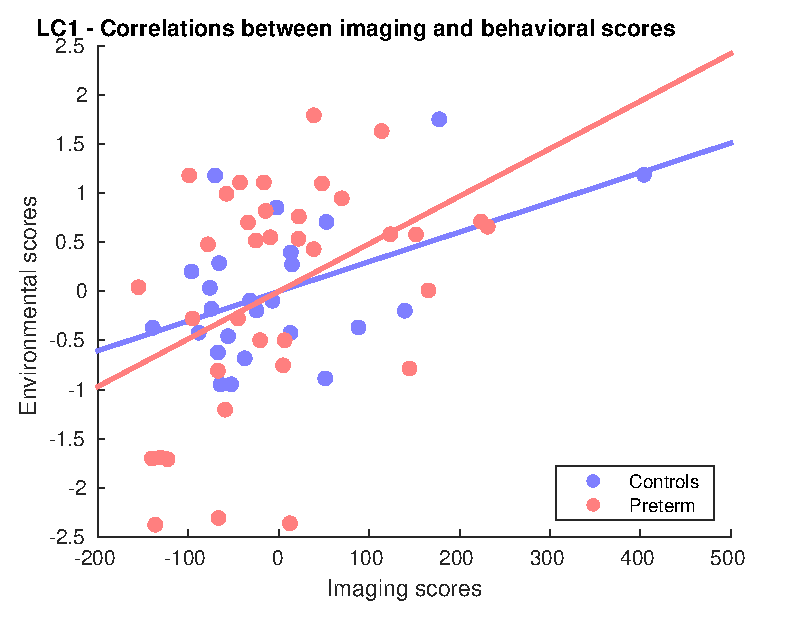
\includegraphics[width=0.8\textwidth]{images/Appendix/ch3_BrainScoresxBehavScores.eps}
\caption{\textbf{Correlation between brain and environmental scores for BOLD variability PLS.}  }
\label{fig:ch3_brainXbehavScores}
\end{figure*}

\begin{figure*}[h]
\centering
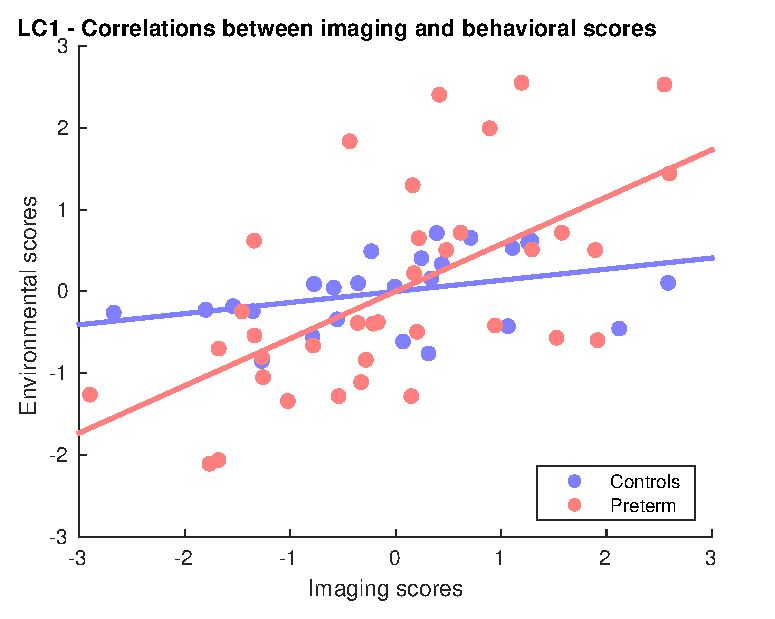
\includegraphics[width=0.8\textwidth]{images/Appendix/ch3_CAPs_BrainScoresxBehavScores.eps}
\caption{\textbf{Correlation between brain and environmental scores for CAP PLS.}  }
\label{fig:ch3_CAP_brainXbehavScores}
\end{figure*}


\chapter{Supplementary material for Chapter \ref{chapter:ch5}} \label{appA}

\renewcommand{\theequation}{Eq. \thechapter.\arabic{equation}}

\section{Link between conventional PPI and the stationary PPI-CAP} 


Within the PPA/CAPs framework, it is well known that averaging the frames where the seed exceeds a ``well chosen'' threshold $\phi$, yields a proxy for the conventional seed connectivity map \citep{Tagliazucchi2012,Liu2013}.
This observation can be explained in the following way:
let us assume that the activity time course $S(t)$ of a seed voxel is a realization over time, $t=1,\ldots,N$, of a random variable $S$ for which $E[S]=0$ and $E[S^2]=1$. 
To construct conventional seed connectivity, a general linear model (GLM) is put forward to explain the time course $V(t)$ of a target voxel as:
\begin{eqnarray}
\label{eqn:ppa_glm}
  V(t) & =& \beta S(t) + \varepsilon(t),
\end{eqnarray}
where $\beta$ is the parameter weight (i.e., functional connectivity) and $\varepsilon(t)$ is the residual and assumed to be a realization of the noise with $E[\varepsilon]=0$ and  $E[\varepsilon^2]=\sigma^2$. In addition, we assume the noise to be independent from the seed voxel activity; i.e., $E[S\cdot \varepsilon]=0$. Multiplying both sides of Eq.~(\ref{eqn:ppa_glm}) with $S(t)$ and taking the expectation leads to:
\begin{eqnarray}
   E[ V  \cdot S ]  & = & \beta E[S^2] + E[S \cdot \varepsilon],
\end{eqnarray}
which simplifies into $\beta=E[V\cdot S]$. 

To obtain the stationary map in the CAPs approach, we want the expectation value of the target voxel for frames where the seed exceeds a threshold $\phi$:
\begin{eqnarray}
  I_\text{CAP+} &=& E[V:S>\phi] \\
          &=& E[\beta S + \varepsilon : S>\phi] \\
          &=& \beta E[S : S>\phi] + E[\varepsilon  : S>\phi],    \label{eqn:ppa-proof}
\end{eqnarray}
where in the first step we have substituted the previous GLM of Eq.~(\ref{eqn:ppa_glm}) and ``$:$" implies conditioning.
Due to the independence of noise and seed voxel, and $E[\varepsilon]=0$, the second term of Eq.~(\ref{eqn:ppa-proof}) will vanish, and we obtain
\begin{equation}
 I_\text{CAP+} = \beta E[S : S > \phi],
\end{equation}
which means that the expectation of suprathreshold frames in the PPA method will be proportional to the result of a conventional correlation map, with the constant of proportionality given by $E[S|S > \phi]$, which only depends on the seed, and not the target voxel. A similar relationship can be derived when the seed activity is below the negative threshold: 
\begin{eqnarray}
  I_\text{CAP-} &=& E[V : S<-\phi] \\
          &=& E[\beta S + \varepsilon : S<-\phi] \\
          &=& \beta E[S : S<-\phi] + E[\varepsilon  : S<-\phi] \\
          &=& \beta E[S : S<-\phi]
\end{eqnarray}
In the case of a two-sided threshold, using the identity $\sign(A)A = |A|$, we can conclude that: 
\begin{eqnarray}
  I_{CAP} &=& E\big[\sign(S)V : \left| S \right|>\phi\big] \\
   &=& E[\beta S\sign(S) + \varepsilon\sign(S) : \left| S \right|>\phi\big] \\
          &=& \beta E[S\sign(S)  : \left| S \right|>\phi\big] + E[\varepsilon \sign(S)  : \left| S \right|>\phi\big] \\
               &=& \beta E\big[|S|\, : \, \left|S \right| > \phi\big].
\end{eqnarray}



Based on this observation, we can generalize to PPI for which the GLM becomes:
\begin{eqnarray}
\label{eqn:ppi_glm}
  V(t) & =& \beta_S S(t) + \beta_T T(t) + \beta_{PPI} P(t) + \varepsilon(t),
\end{eqnarray}
where $T(t)$ is the time course of the task and $P(t)$ is the ``interaction term'' given by $P(t) = S(t)T(t)$. The stationary map of the PPI-CAPs analysis then averages values of the target voxel multiplied with the sign of the interaction term, where the selection is based on the criterion of the seed exceeding the threshold: 
\begin{eqnarray*}
   I_\text{PPI-CAP} & = & E[ \sign(ST) V : \left| S\right|>\phi] \\
   & = & E[ \sign(ST) ( \beta_S S + \beta_T T + \beta_{PPI} P + \varepsilon) : \left| S\right| >\phi] \\
   & = & \beta_S E[ \sign(ST) S : \left| S \right|>\phi] + \beta_T E[\sign(ST) T : \left| S \right|>\phi] + \beta_{PPI} E[\sign(ST) P : \left| S \right| > \phi].
\end{eqnarray*}
Using the identities $\sign(A)A = |A|$ and $\sign(AB)A = \sign(B) |A|$, this becomes
\begin{eqnarray*}
  I_\text{PPI-CAP} &= & \beta_S E\big[\sign(T)|S| : \left| S\right|>\phi\big] + \beta_T E\big[\sign(S)|T| : \left| S\right|>\phi\big] \label{eqn:ppi-T-term} + \beta_{PPI} E\big[|ST| : \left| S\right|>\phi\big] \\
  & \approx & \beta_{PPI} E\big[|ST| : \left| S\right|>\phi\big].
\end{eqnarray*}
The last approximation can be made when the contributions of the first two terms are negligible. 
For the first term, we assume the absolute value of $S$ to be independent of the task (that weights the expectation operator) and $T$ has equal number of positive and negative values, in which case the first term will be 0. 
For the second term, if the task is just a change of sign, then its absolute value will be fixed and uncorrelated to the sign of the seed. Thus the second term is proportional to $E\big[\sign(S) : \left| S\right|>\phi\big]$, which is necessarily bound between $\pm1$ and will be exactly 0 if S is symmetric.

Therefore, what remains is the final term and we find that the result of a PPI analysis will be proportional to the SiMap.
This brief derivation also shows that the stationary PPI-CAP can be contaminated by ``leakage'' from the seed and/or task contributions if these assumptions are not fulfilled. 


\clearpage
\section{Supplementary Figures for Section \ref{section:ppicaps_method}} \label{Supp}

% Reset Figure count
%\setcounter{figure}{0}



\begin{figure*}[h]
\centering
\includegraphics[width=1\textwidth]{Appendix/20191120_simapIntuition.pdf}
\caption{\textbf{An intuitive toy example to illustrate the relationship between the static interaction map (simap) and PPI analysis results.} A)~Moments where the seed activity is significantly high (red stars) or low (blue stars) are selected. B)~Three possible cases are depicted: 1)~When the target voxel is correlated only with the seed (meaning that there is no interaction effect), its resulting value in the siMap will be close to zero, as would be expected for its corresponding beta value in a PPI analysis. 2)~Similarly, when the target voxel is correlated only with the task, its resulting value in the siMap will be close to zero. 3)~when the target voxel is correlated with the PPI regressor, meaning that its relationship with the seed changes according to the context, the averaged value from its suprathreshold frames will yield a high value, indicating a PPI effect.}
\label{fig:simapIntuition}
\end{figure*}


\begin{figure*}[h]
\centering
\includegraphics[width=1\textwidth]{Appendix/20191201_SeedChecks.pdf}
\caption{\textbf{Sanity check on the chosen seed signal.} Before proceeding with the PPI-CAPs analysis, we checked the orthogonality of the seed, task and ppi regressors using SPM's Check Orthogonality tool, as well as the skewness of the seed. A)~The group-averaged matrix confirms that the regressors are not collinear at the group level. The highest off-diagonal value is 0.04. B)~Shows the same matrix at the single-subject level. C)~The seed signal was not skewed for any of the subjects: the skewness value stayed within the [-0.5 0.5] range for all of them. D)~Shows the distribution of z-scored seed signal values for each subject. Additionally, the magnitude of the seed timecourse was not correlated with the sign of the task: the Pearson’s r coefficient for the subject with the strongest correlation between the magnitude of the seed and the sign of the task was 0.11.  }\label{fig:seedcheck}
\end{figure*}

\begin{figure*}[h]
\centering
\includegraphics[width=0.5\textwidth]{Appendix/20190810_GroupMap}
\caption{\textbf{Group-level static interaction map resembles PPI analysis results.} The spatial correlation betweeen the two analyses' results was 0.85 for the siMap calculated from 60\% frames. }
\label{fig:groupSimap}
\end{figure*}


\begin{figure*}[h]
\centering
\includegraphics[width=1\textwidth]{Appendix/20190809_ConsensusClustering}
\caption{\textbf{An analysis of the number of occurrences of each PPI-CAP per subject combined with consensus clustering indicates the optimal number of groups in which to cluster the suprathreshold frames.} (Top) The PPI-CAPs distributions for  $k\in[3, 8]$ showed that $k$ values of 6 and above yielded PPI-CAPs that never occurred for some subjects, while values between 4 and 5 had the most homogeneous distribution of pattern occurrence per subject. (Bottom) Visual inspection of the consensus matrices showed that the most stable values for $k$ (that is, those for which any two frames would most consistently be clustered together or separately) were $k=3$ and $k=4$. Since 4 represents a better trade-off in terms of variety and robustness, we chose this value for further analysis (see its clear pattern highlighted in green). The colormap represents the proportion of time when two frames were consistently clustered either together or separately.}
\label{fig:consensus}
\end{figure*}

\begin{figure*}[h]
\centering
\includegraphics[width=1\textwidth]{Appendix/20191120_stats.pdf}
\caption{\textbf{Significance assessment of PPI-CAPs.} Each histogram illustrates the distribution of determinant values of the confusion matrices obtained from 3000 random permutations of the frame labels composing each PPI-CAP, with respect to seed, task or PPI. The red line indicates where the determinant of the confusion matrix for real data lies.  }
\label{fig:permanova}
\end{figure*}



\begin{figure*}[h]
\centering
\includegraphics[width=1\textwidth]{Appendix/20190809_PPI_CAPs_Fig5}
\caption{\textbf{The high temporal resolution of the PPI-CAPs approach allows us to link brain activity to stimuli presented at specific time points.} Here, we show moments when each PPI-CAP was highly consistent across participants (left). The y-axis shows the percentage of subjects, out of the total 15 participants, who expressed the PPI-CAP at each given time point.  The histogram on the right hand side of the panel depicts the distribution of random consistency across subjects. This was calculated by randomly permuting the time points on which the PPI-CAP appeared for each subject, then re-calculating the subject consistency across time (the same plot as the ones on the left). Finally, we plotted the distribution of possible consistency values. The dashed line represents the value of the 99\textsuperscript{th} percentile from the random distribution, indicating that a subject consistency above this threshold is significant. Selected time points of high consistency across subjects for each PPI-CAP are indicated by numbers on the left plots, and the corresponding video frames are presented for those times on the rightmost side of the figure.   }
\label{fig:PPI_CAPs_Fig5}
\end{figure*}


\clearpage
\section{Supplementary Figures for Section \ref{section:ppicaps_preterm}}

\subsection{ACC-seed PPI-CAPs in preterm-born adolescents}
% --------------------------------------------------------------------------
% ACC-SEED CHOICE OF K
% --------------------------------------------------------------------------


\begin{figure*}[h]
\centering
\includegraphics[width=1\textwidth]{images/Appendix/Appendix_Ch4_ACC_K.png}
\caption{\textbf{Choosing the best number of clusters for an ACC-seed PPI-CAPs analysis.} 30\% of the frames when the dorsal anterior cingulate cortex (ACC) was most (de)activated were selected for analysis. Consensus clustering was run for K ranging from 3 to 20, in 10 folds for each of which a random subsample including 80\% of the subjects was used. On the left, the consensus matrices provide a visual appreciation of how often each pair of frames was consistently clustered (\textit{i.e.,} both always in the same cluster, or both never in the same cluster). Blue indicates never, red indicates always. On the right, we plot the proportion of ambiguously clustered frames for each K. Since we want this value to be very low, a peak in the (1-PAC) plot indicates the most stable choice of K. Since K~=~6 has a clear peak and means we will have a large number of frames per PPI-CAP (essential for averaging out noise), we select this as opposed to higher K numbers who also had good results.}
\label{fig:app_acc_k}
\end{figure*}




% --------------------------------------------------------------------------
%  ACC PPI-CAPS ASSINMENT TO YEO NETWORKS
% --------------------------------------------------------------------------

\begin{figure*}[h]
\centering
\includegraphics[width=1\textwidth]{images/Appendix/ACCK6_assigment_YeoRSN.png}
\caption{\textbf{Identifying networks present in each PPI-CAP.} The two matrices compare the activated (red) and deactivated (blue) voxels in each PPI-CAP from Figure \ref{fig:acc_ppicaps} to the 7 functional networks from \citet{Yeo2011}. Colour intensity and numbers indicate the proportion of voxels from each network that are present in the PPI-CAP. Networks were then ordered according to the Hungarian Assignment Algorithm \citep{Munkres1957}. According to this result, PPI-CAP\textsubscript{1} corresponds to an activated Somatomotor Network (SMN) and deactivated Default Mode Network;  PPI-CAP\textsubscript{2} is assigned to an activated Ventral Attention Network, also known as Salience Network (SN),  and deactivated Limbic; PPI-CAP\textsubscript{3} contains an activated Visual and deactivated Frontoparietal Network (FPN); PPI-CAP\textsubscript{4} includes an activated Dorsal Attention (DAN) and deactivated Visual Network; PPI-CAP\textsubscript{5} has an activated FPN and deactivated SMN; and PPI-CAP\textsubscript{6} includes an activated Limbic and deactivated DAN.  }
\label{fig:app_acc_munkres}
\end{figure*}





% --------------------------------------------------------------------------
%  ACC-based PERMUTATION TESTING
% --------------------------------------------------------------------------


\begin{figure*}[h]
\centering
\includegraphics[width=1\textwidth]{images/Appendix/ACCK6_stats_permutation2.png}
\vspace{5mm}
\caption{\textbf{Statistical assessment of each PPI-CAP's effects.} To check whether the effects identified in Figure \ref{fig:acc_cm} are significant, we performed permutation testing by shuffling the corresponding effect's labels 3000 times and calculating the det-index in each case, to generate a null distribution. We then check where the real data's det-index lies within this distribution and calculate the p-value. }
\label{fig:app_acc_stats}
\end{figure*}







% --------------------------------------------------------------------------
%  PCC SECTION
% --------------------------------------------------------------------------

\clearpage
\subsection{PCC-seed PPI-CAPs in preterm-born adolescents} \label{sm_pcc_ppicaps}
 In Chapter \ref{chapter:ch5}, Section \ref{section:ppicaps_preterm}, we perform a PPI-CAPs analysis to explore task-related dynamic connectivity using the dorsal anterior cingulate cortex as a seed. Here we provide a similar analysis using the posterior cingulate cortex (PCC). While interpreting these additional results goes beyond the goal of this Section, this additional work illustrates that task-driven dynamics are a powerful and compelling strategy to uncover features of brain function in clinical populations independently of the choice of seed. 
\vspace{1cm}




% --------------------------------------------------------------------------
% PCC-SEED CHOICE OF K
% --------------------------------------------------------------------------


\begin{figure*}[h]
\centering
\includegraphics[width=1\textwidth]{images/Appendix/Appendix_Ch5_PCC_K.png}
\caption{\textbf{Choosing the best number of clusters for a PCC-seed PPI-CAPs analysis.} 30\% of the frames when the posterior cingulate cortex (PCC) was most (de)activated were selected for analysis. Consensus clustering was run for K ranging from 3 to 20, in 10 folds for each of which a random subsample including 80\% of the subjects was used. On the left, the consensus matrices provide a visual appreciation of how often each pair of frames was consistently clustered (\textit{i.e.,} both always in the same cluster, or both never in the same cluster). Blue indicates never, red indicates always. On the right, we plot the proportion of ambiguously clustered frames for each K. Since we want this value to be very low, a peak in the (1-PAC) plot indicates the most stable choice of K. Since K = 4 has a clear peak and means we will have a large number of frames per PPI-CAP (essential for averaging out noise), we select this as opposed to higher K numbers who also had good results.}
\label{fig:app_pcc_k}
\end{figure*}

% --------------------------------------------------------------------------
% PCC-SEED PPI-CAPS
% --------------------------------------------------------------------------

\begin{figure*}[h]
\centering
\includegraphics[width=0.85\textwidth]{images/Appendix/Appendix_Ch5_PPI-CAPs.pdf}
\caption{\textbf{PCC-seed PPI-CAPs.} Using K~=~4 for the clustering step as defined in Figure \ref{fig:app_pcc_k} yielded the four PPI-CAPs above. Each row corresponds to one PPI-CAP, numbers indicate slice coordinates in MNI space.}
\label{fig:app_pcc_ppicaps}
\end{figure*}


% --------------------------------------------------------------------------
%  PCC PPI-CAPS ASSINMENT TO YEO NETWORKS
% --------------------------------------------------------------------------

\begin{figure*}[h]
\centering
\includegraphics[width=1\textwidth]{images/Appendix/PCCK4_assigment_YeoRSN.png}
\caption{\textbf{Identifying networks present in each PPI-CAP.} The two matrices compare the activated (red) and deactivated (blue) voxels in each PPI-CAP from Figure \ref{fig:app_pcc_ppicaps} to the 7 functional networks from \citet{Yeo2011}. Colour intensity and numbers indicate the proportion of voxels from each network that are present in the PPI-CAP. Networks were then ordered according to the Hungarian Assignment Algorithm \citep{Munkres1957}. According to this result, PPI-CAP\textsubscript{1} corresponds to an activated Dorsal Attention Network (DAN) and deactivated Default Mode Network;  PPI-CAP\textsubscript{2} is assigned to an activated Limbic Network (LN) and deactivated DAN; PPI-CAP\textsubscript{3} contains an activated Salience Network and deactivated LN; and PPI-CAP\textsubscript{4} includes an activated Visual Network and deactivated Fronto-Parietal Network. }
\label{fig:app_pcc_munkres}
\end{figure*}




% --------------------------------------------------------------------------
%  PCC-based CONFUSION MATRICES
% --------------------------------------------------------------------------


\begin{figure*}[h]
\centering
\includegraphics[width=1\textwidth]{images/Appendix/PCCK4_PPICAPs_confusionMatrices.png}
\vspace{5mm}
\caption{\textbf{Confusion matrices for PCC-seed PPI-CAPs.} To identify main and interaction effects for each PPI-CAP, we generate confusion matrices to see how often the sign of a PPI-CAP switches in the same way as each of the effects. We tested three main effects (Seed; Task; and Group) and three interaction effects (Seed vs. Task (PPI); Group vs. Seed; and Group vs. Task). The signs for each effect are as follows: Seed --- positive and negative signs correspond to frames when the seed was activated of deactivated, respectively;  Task --- positive signs correspond to "Movie Watching" while negative signs correspond to moments of "Emotion Regulation"; Group --- positive signs correspond to fullterm controls, while negative signs correspond to preterm-born individuals. Interaction signs are calculated as element-by-element multiplication of the main effect signs. Light yellow indicates a low number of frames, while dark red indicates the highest number of frames. }
\label{fig:app_pcc_confusion}
\end{figure*}



% --------------------------------------------------------------------------
%  PCC-based PERMUTATION TESTING
% --------------------------------------------------------------------------


\begin{figure*}[h]
\centering
\includegraphics[width=1\textwidth]{images/Appendix/PCCK4_stats_permutation.png}
\vspace{5mm}
\caption{\textbf{Statistical assessment of each PPI-CAP's effects.} To check whether the effects identified in Figure \ref{fig:app_pcc_confusion} are significant, we performed permutation testing by shuffling the corresponding effect's labels 3000 times and calculating the det-index in each case, to generate a null distribution. We then check where the real data's det-index lies within this distribution and calculate the p-value. }
\label{fig:app_pcc_stats}
\end{figure*}